\documentclass[10pt]{exam}
\usepackage[hon]{template-for-exam}
\usepackage{tikz,graphicx}
\usetikzlibrary{shadings,decorations.pathmorphing,arrows.meta,patterns}

\title{Conservation of Momentum Consolidation.}
\author{Rohrbach}
\date{\today}

\begin{document}
\maketitle

\begin{questions}
  
\question
  Consider the folowing objects that collide on a frictionless surface.  If $m_A=4$ kg and $m_B=1$ kg, what is the final velocity of object A?

  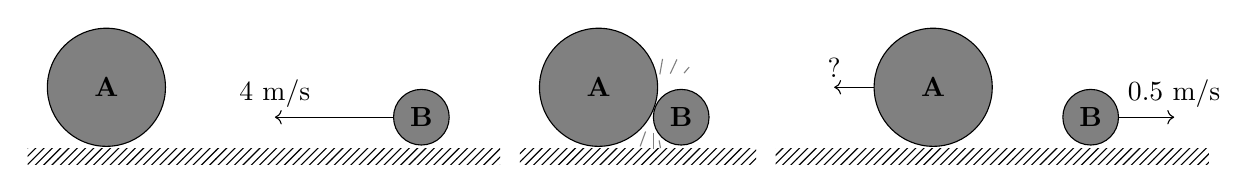
\begin{tikzpicture}
    \begin{scope}
      \node
        [circle, minimum size=1.5cm, fill=gray, draw=black] 
        at (0,.38) (A) {\bf A};
      \node[circle, fill=gray, draw=black] 
        at (4,0) (B) {\bf B};
      \draw[->] (B.west) -- ++(-1.5,0) 
        node[above] {4 m/s};
      \fill[pattern=north east lines]
        (-1,-0.4) rectangle ++(6,-0.2);
    \end{scope}

    \begin{scope}[shift={(6.25,0)}]
      \node
        [circle, minimum size=1.5cm, fill=gray, draw=black] 
        at (0,.38) (A) {\bf A};
      \node[circle, fill=gray, draw=black] 
        at (1.05,0) (B) {\bf B};
      \fill[pattern=north east lines]
        (-1,-0.4) rectangle ++(3,-0.2);

        \begin{scope}[shift={(.7,.1)},gray]
          \draw[] (50:.6) -- ++(50:.1);
          \draw[] (65:.5) -- ++(65:.2);
          \draw[] (80:.45) -- ++(80:.2);
          \draw[] (-80:.4) -- ++(-80:.1);
          \draw[] (-90:.3) -- ++(-90:.2);
          \draw[] (-110:.3) -- ++(-110:.2);
        \end{scope}
    \end{scope}

    \begin{scope}[shift={(9.5,0)}]
      \node
        [circle, minimum size=1.5cm, fill=gray, draw=black] 
        at (1,.38) (A) {\bf A};
      \node[circle, fill=gray, draw=black] 
        at (3,0) (B) {\bf B};
      \draw[->] (B.east) -- ++(.7,0) 
        node[above] {0.5 m/s};
      \draw[->] (A.west) -- ++(-.5,0) 
        node[above] {?};
      \fill[pattern=north east lines]
        (-1,-0.4) rectangle ++(5.5,-0.2);
    \end{scope}
  \end{tikzpicture}

  \vs

\question
  A 1500-kg truck traveling at 15~m/s rear-ends a stationary 900-kg car.  After the collision, the two vehicles stick together.  Before friction has a chance to take effect, what is the speed of the cars?
  \vs

\question
  A 900-kg cannon fires a 5-kg cannonball at a speed of 30~m/s.  What is the speed of the cannon's recoil?
  \vs

\end{questions}

\end{document}